\chapter{Introdución}
\label{chap:introducion}

\lettrine{E}{ste} proxecto busca crear un simulador de RISC-V empregando a libraría SystemC en C++. Ao longo desta memoria describiranse as etapas de execución, as extensións e os distintos módulos, así como a motivación destes.

 - agradecementos

\section{Motivación}
\label{sec:motivación}
RISC-V apunta a ser unha das arquitecturas máis empregadas nun futuro, xa que é libre, permitindo aforrar o custo de licenzas. Grazas a que se pode modificar, engadindo ou eliminando funcionalidades, isto permite que abarque múltiples sectores, dende \gls{chips} máis sinxelos orientados a \acrfull{iot}, ata competir con \acrshort{arm} en sistemas embebidos ~\cite{RISCV_IoT,RISCV_vsARM}. Co nacemento da nova \acrfull{isa} debido á necesidade dun conxunto de instrucións máis sinxelo e sen custos por licenzas, nace a necesidade de crear un simulador adaptado tanto a esta \acrshort{isa} como á arquitectura RISC-V. Se ben xa existen varios simuladores, cada un está especializado nun rango de aplicacións, e consideramos que a simulación orientada a unha implementación posterior non está suficientemente cuberta. Así, simuladores como RARS ~\cite{rars} ou Spike ~\cite{sim_spike} son especialmente útiles na docencia ou valoracións da arquitectura. Por outra banda, RISC-V-TLM ~\cite{riscv_tlm} funciona a un nivel moi superior, simulando a nivel de transferencias, e permite unha simulación de sistemas completos aínda que relaxando moito a precisión temporal. Por último, Chisel ~\cite{chisel} está baseado en Scala, e permite o modelado de circuítos dixitais. A relevancia de Chisel é que foi utilizado no desenvolvemento de RISC-V, ademais de que permite xerar automáticamente código Verilog simulable e sintetizable.

As vantaxes de empregar SystemC son o control absoluto sobre todo os aspectos do modelado, a velocidade de simulación, e a facilidade para depurar o código ao estar baseado en C++.

Durante o proceso de deseño, unha parte clave é a verificación do correcto funcionamento ~\cite{ChipVerify_verification,RISCV_verification}. Debido ao elevado custo de fabricación, e ao tempo necesario (ao redor de 3 meses), é inviable crear un chip para cada versión. Ahí é onde un simulador toma protagonismo, xa que permite probar de forma rápida, sinxela e barata os deseños creados. Ademais, é unha ferramenta moi interesante para as investigacións da comunidade científica e incluso para entornos educativos.

\section{Obxectivos}
\label{sec:obxectivos}
Os obxectivos deste proxecto son modelar e simular, usando SystemC, as seguintes extensións da arquitectura RV32I: 

\begin{itemize}
    \item multiplicación e división por números enteiros (extensión M).
    \item aritmética en punto flotante de simple (extensión F).
    \item xestión de rexistros de control e estado (extensión Zicsr).
    \item sincronización de escritura de instrucións (extensión Zifencei).
\end{itemize}

O modelado será totalmente parametrizable, permitindo especificar a latencia das diferentes instrucións. Tamén permitirá especificar o número de canles de execución para as unidades de enteiros a punto flotante, e se estes están ou non totalmente segmentados. 

Desta maneira, a simulación permitirá comparar o rendemento de, por exemplo, unha implementación na que o multiplicador e o divisor comparten circuítos, cunha na que ambos son independentes, e tamén comparar un divisor totalmente segmentado cun que non o sexa. 

Os resultados do modelado e a simulación son dous: verificar o correcto funcionamento da arquitectura e comprobar o seu rendemento. 


\section{Metodoloxía}
\label{sec:metodoloxía}
O método de traballo foi incremental, dividindo as tarefas en partes independentes que foron implementadas, simuladas e verificadas por orde de complexidade antes de proceder coa seguinte.

O procedemento habitual foi dunha reunión semanal na que se revisaba o feito anteriormente, acompañado de comprobación cos tests correspondentes para esa parte. Despois, decidíase cal era o seguinte paso, podendo ser a implementación dunha nova extensión ou modificar un módulo do simulador.

\subsection{Fases principais}
\begin{itemize}
    \item Estudio da documentación existente sobre RISC-V.
    \item Familiarización coa implementación base de RV32I en SystemC. 
    \item Modelado e simulación do multiplicador e divisor de enteiros. 
    \item Modelado e simulación das extensións de punto flotante F e D. 
    \item Modelado e simulación de extensións Zicsr e  Zifencei.
    \item Empaquetamento do software. 

\end{itemize}

En canto á organización do proxecto, establecéronse unhas tarefas básicas a realizar. Creouse un plan inicial, como foi explicado no anteproxecto. Sen embargo, non se puido cumprir na súa totalidade pola subestimación do tempo necesario para completar ditas actividades. Como consecuencia disto, a implementación das extensións A e D non puido ser realizada. 

En canto ó seguimento do proxecto, creouse un diagrama de Gantt coas actividades a realizar, que se foi actualizando para eliminar as descartadas. 

\begin{figure}[hp!]
  \centering
  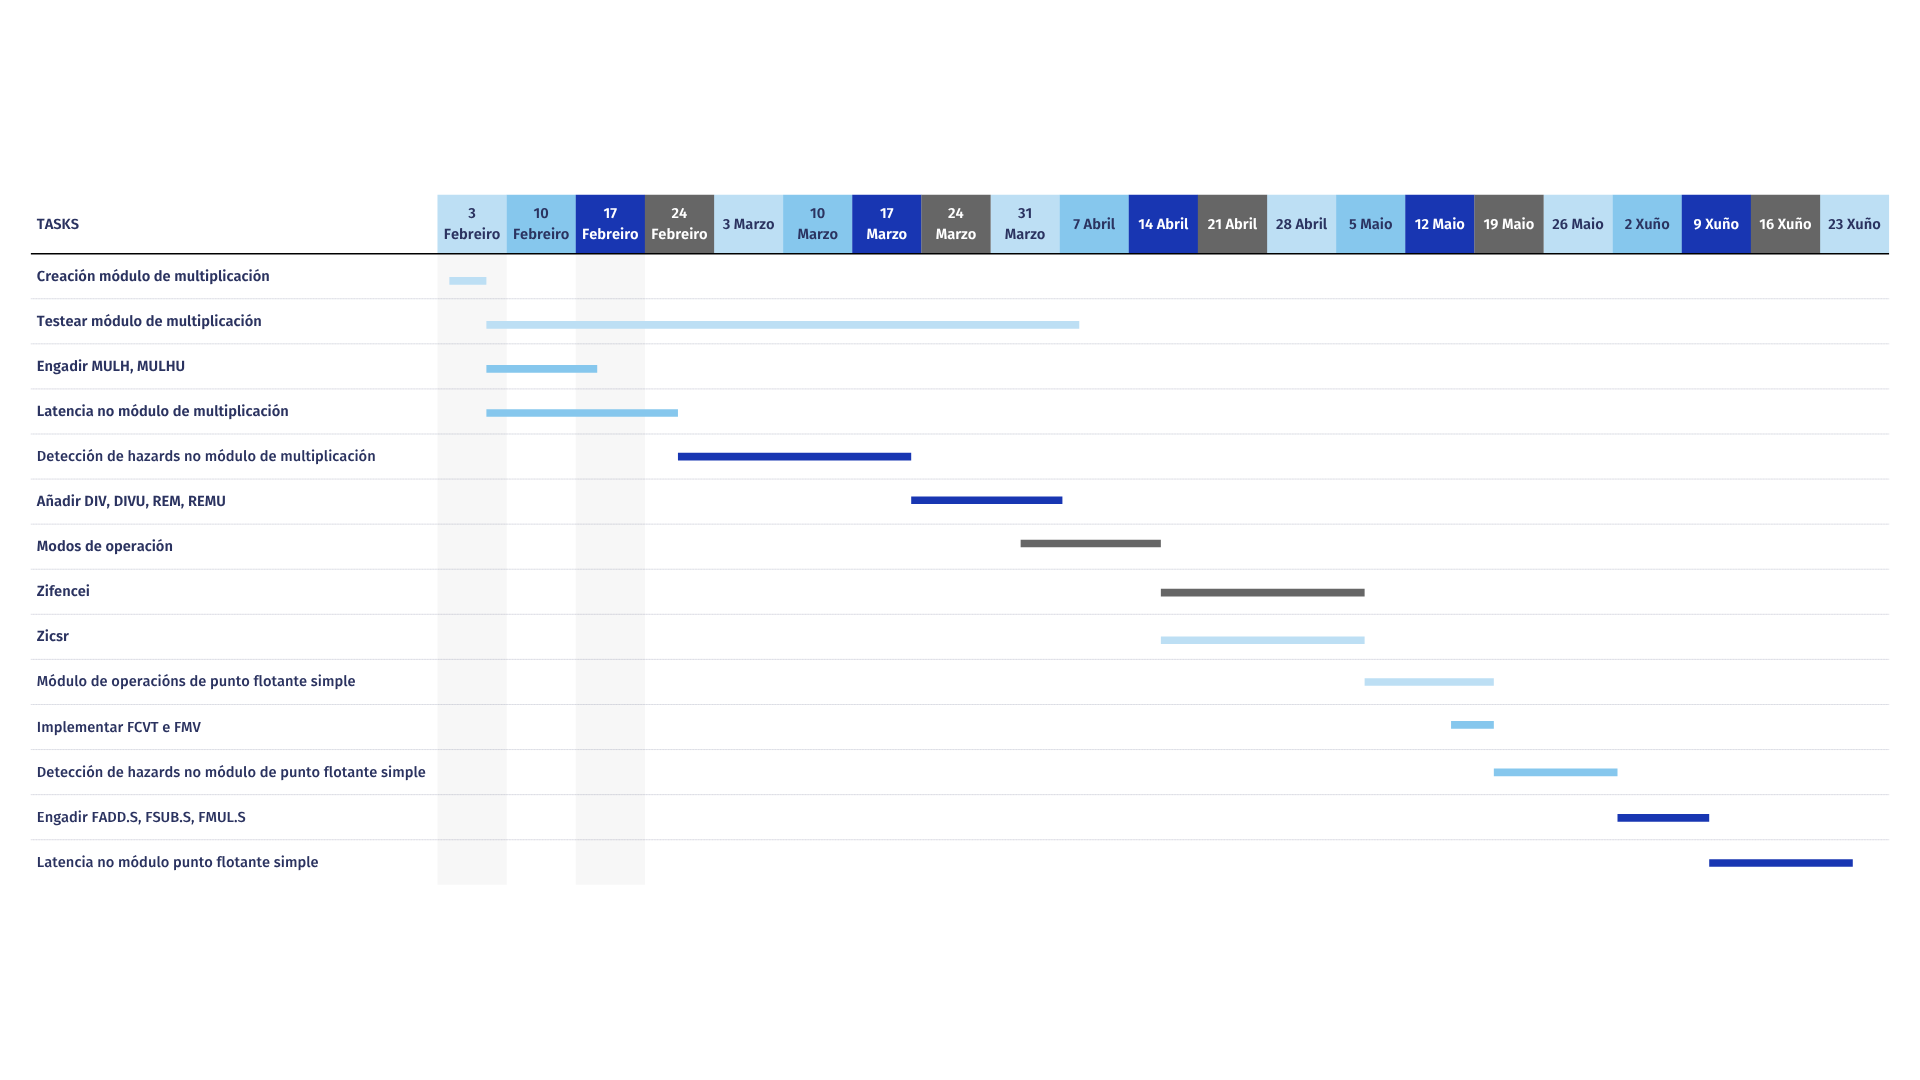
\includegraphics[width=\textwidth]{imaxes/Gantt - TFG.png}
  \caption{Esquema sobre o pipeline do módulo de multiplicación.}
  \label{fig:gantt}
\end{figure}

\section{Contida da memoria}
\label{sec:contido_memoria}
Nesta sección describirase brevemente os capítulos desta memoria e o seu contido: 
\begin{itemize}
    \item \textbf{Capítulo 1: Introducción.}  O primeiro capítulo inclúe unha descrición sobre o proxecto, cal foi a motivación deste, os obxectivos propostos para este traballo e a metodoloxía empregada.
    \item \textbf{Capítulo 2: RISC-V.} Aqui falarase sobre a arquitectura, explicando as súas características máis interesantes, as extensións e outros datos relevantes.
    \item \textbf{Capítulo 3: Modelación e simulación} Explicación sobre que é o modelado e a simulación, por qué son útiles e as linguaxes máis empregadas.
    \item \textbf{Capítulo 4: Deseño do simulador.} Neste capítulo tratarase os distintos módulos creados, o por qué e as decisións de deseño detrás destas.
    \item \textbf{Capítulo 5: Implementación.} Explicarase as ferramentas empregadas, como se aplicou a metodoloxía e o proceso de engadir as extensións.
    \item \textbf{Capítulo 6: Probas.} Neste quinto apartado detallase o procedemento para comprobar o correcto funcionamento do simulador, como se elaboraron os tests, unha breve explicación de como funcionan e os programas empregados para a depuración.
    \item \textbf{Capítulo 7: Uso do simulador.} Contén unhas breves indicacións de como empregar o software.
    \item \textbf{Capítulo 8: Conclusións.}
    \item \textbf{Apéndices. }
    \item \textbf{Bibliografía. }
    
\end{itemize}

